

\section{Gibbs}
\label{chap:gibbs}

Figure \ref{fig:gibbs_quality} shows the dependency between quality of the chains and model complexity.  Interestingly, we observe that quality does \textit{not} decrease as the model complexity (i.e. parameters to estimate) increases. 

Unsurprisingly, the greater the sample size, the closer the estimates are to the original model. Note, however, that sampling size $500$ appears to be an exception, as - for those benchmarks - it produces solutions of about equal quality as for higher sample sizes. This can be explained by the fact that for simple models, small sample sizes are sufficient and for more complex models, Gibbs's sampler for small sample sizes simply does often not converge. This is illustrated in figure \ref{fig:gibbs_convergence}. So, \textit{if} the Gibb's sampler converges for a small sample size, its quality is good. However, for more complex models, it does not (sufficiently) converge in the first place. 
Please note that in figure \ref{fig:gibbs_quality}, only chains which have converged (i.e. the algorithm aborted before reaching $3,000$ elements) have been considered. 

This begs the question whether small sample sizes should be used at all. Figures \ref{fig:gibbs_quality} as well as \ref{fig:gibbs_runtime} provide the relevant information: While a smaller sample sizes yield a stationary distribution faster, when taking into account the empirically obtained  convergence rates, the advantages in terms of time spent do not outweigh the inferiority in convergence rates. Note in particular that the algorithm failed to converge for any of the $3\times3 =9$ runs for the full $6$ parameter model if a sample size of only $500$ was used. Note that this may be due more because of \textit{unidentifiability} of the model than because of a shortcoming of the algorithm or implementation itself. 

\begin{figure}
	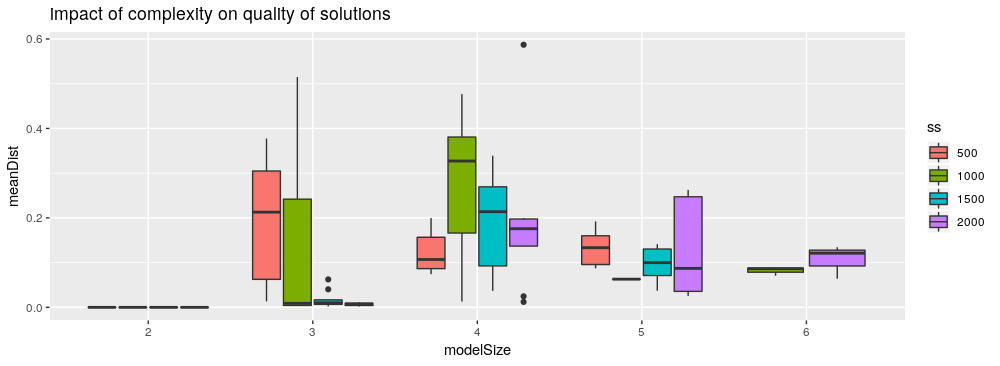
\includegraphics[width=\linewidth]{img/sim_bern_gibbs_quality.png}
	\caption{MeanDist is defined as the minimum Manhattan distance ($L_1(\R)$) between $\delta$ of the model sampled from and the mean from the last third of the chain after convergence. Generally speaking, more samples produce solutions of higher quality }
	\label{fig:gibbs_quality}
\end{figure}


\begin{figure}
	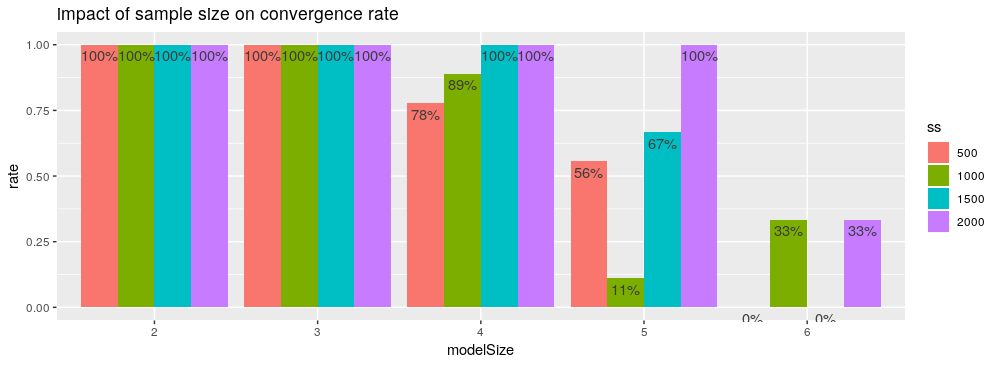
\includegraphics[width=\linewidth]{img/sim_bern_gibbs_convergence.png}
	\caption{Convergence is defined as the max difference inquantiles between the second and third part of the chain falling below the threshold of $0.1$ for the quantiles $0.25, 0.5$ and $0.75$. More complex models yield lower convergence rates; the cut-off point is $3,000$ samples. }
	\label{fig:gibbs_convergence}
\end{figure}


\begin{figure}
	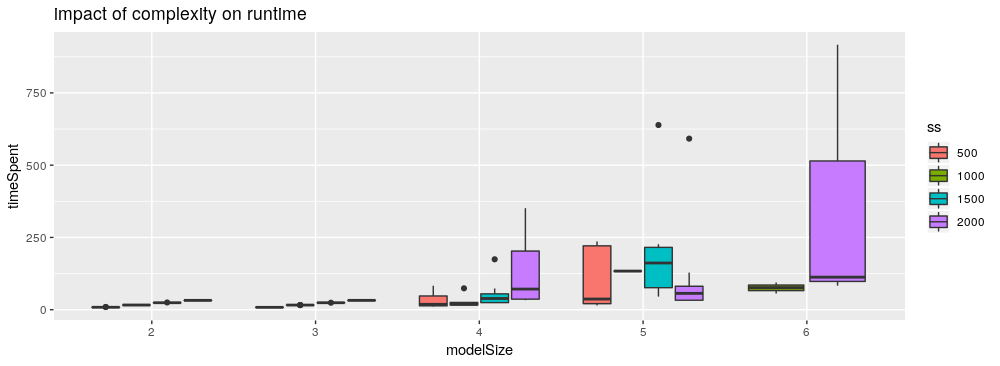
\includegraphics[width=\linewidth]{img/sim_bern_gibbs_runtime.png}
	\caption{The more complex the model, the more time the Gibb's sampler's chain needs until convergence. Missing bars indicate non-convergence of respective chains. }
	\label{fig:gibbs_runtime}
\end{figure}


Figure \ref{fig:gibbs_iterations} shows inconclusive evidence that more samples decrease the number of iterations necessary. 
Note that increasing sample sizes increase the duration of each iteration (at the magnitude of $\mathcal{O}(T)$). On the other hand, more samples increase \textit{identifiability} of the model, which make each step more informative and could reduce the number of iterations necessary. Hence the time spent until convergence does not directly translate into iterations computed.

TODO: include data for model of complexity 7-10

So while figure \ref{fig:gibbs_quality} clearly shows that the quality of the estimation increases with increasing sample size, figure \ref{fig:gibbs_iterations} also shows that still more iterations are needed. 


\begin{figure}
	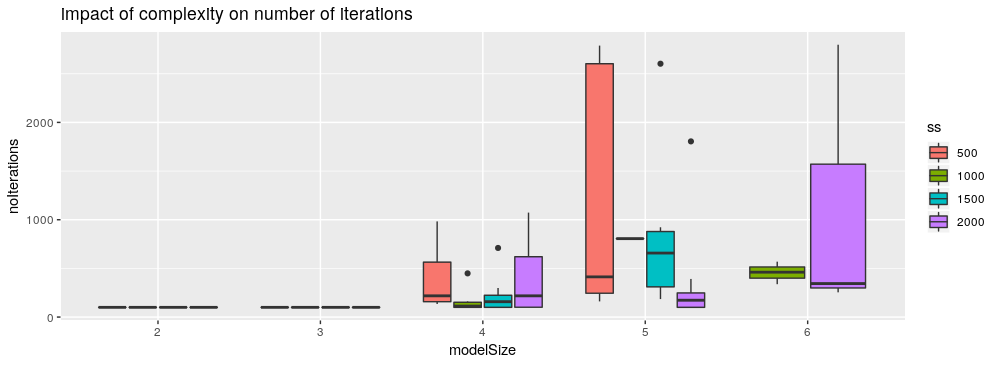
\includegraphics[width=\linewidth]{img/sim_bern_gibbs_iterations.png}
	\caption{More complex models cause longer chains, but more samples also cause longer chains }
	\label{fig:gibbs_iterations}
\end{figure}



\section{Metropolis-Hastings}
\label{chap:mh}

Figure \ref{fig:mh_quality} shows that the quality of the solutions decreases when the model complexity increases. Note how this is markedly different from the Gibb's sampler's results. Generally speaking, the graphs exhibit much more variation, which is due to the relatively small sample size of $3$ models with each $3$ runs. Already judging from this figure, we can see that running several chains with Metropolis Hastings in parallel to decrease variance is a good option.

Figure \ref{fig:mh_runtime} shows that the run time of Metropolis-Hastings is generally lower than of the respective Gibb's sampler. However, more samples seem to have a \textit{negative} effect on the runtime. This suggests that in the setup used in this thesis, the data is not sufficiently informative for the Metropolis-Hastings steps. 

Also note that no chains for model complexity $6$ are shown. This is because none of the chains have converged within the given limit of iterations ($3,000$); this fact is corroborated by figure \ref{fig:mh_convergence}.  All of these effects are not because the chain actually fails to converge towards a stationary distribution; it just does not do so within the time constraint given. This has been verified by manual inspection. That the time limit is quickly reached for complex models becomes evident when examining figure \ref{fig:mh_iterations}; When naiively extrapolating the number of iterations depicted therein, we can clearly see that for a model with $6$ three parameters, the limit of $3,000$ chain samples is quickly exhausted. 


\begin{figure}
	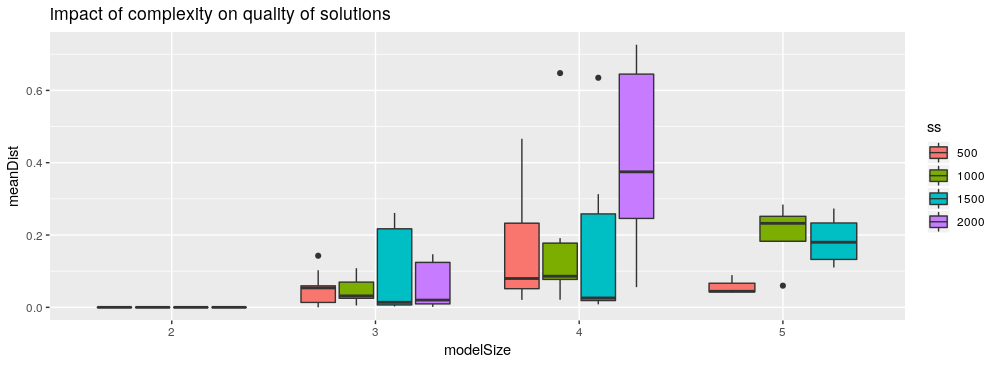
\includegraphics[width=\linewidth]{img/sim_ben_mh_quality.png}
	\caption{Solution quality decreases as model complexity increases; behaviour is highly erratic and model takes very long to converge. No chain converged for the full model given the time constraints.}
	\label{fig:mh_quality}
\end{figure}



\begin{figure}
	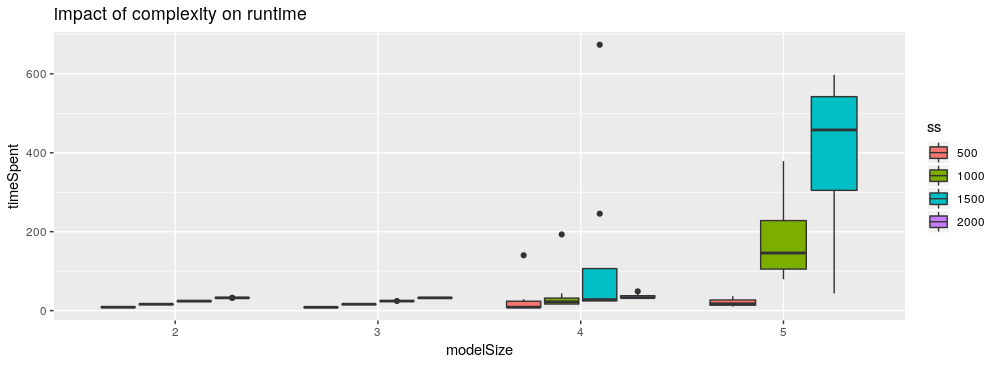
\includegraphics[width=\linewidth]{img/sim_ben_mh_runtime.png}
	\caption{Runtime increases dramatically with model complexity and appers to rise exponentially in terms of sample size}
	\label{fig:mh_runtime}
\end{figure}


\begin{figure}
	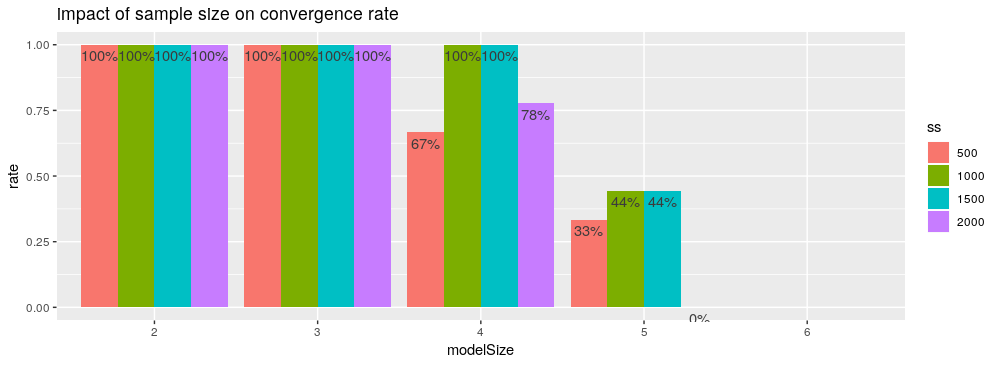
\includegraphics[width=\linewidth]{img/sim_ben_mh_convergence.png}
	\caption{Convergence rates decrease dramatically as model complexity increases; this is due to the number of iterations being limited to $3,000$.}
	\label{fig:mh_convergence}
\end{figure}


\begin{figure}
	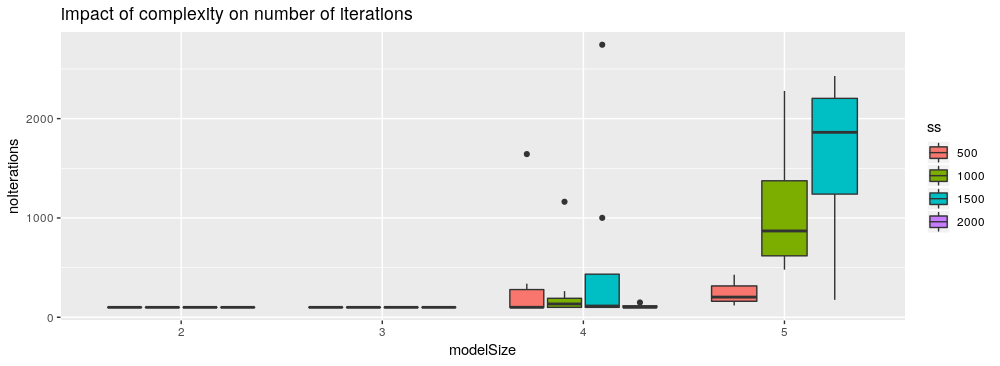
\includegraphics[width=\linewidth]{img/sim_ben_mh_iterations.png}
	\caption{The number of iterations needed increases with model complexity; it also increases excessively with the number of samples}
	\label{fig:mh_iterations}
\end{figure}